% Slide thuyết trình sản phẩm – Nhóm 2, đề tài 16. Đi kèm kịch bản docs/KICH-BAN-THUYET-TRINH.md (10 phút).
% Biên dịch (cần XeLaTeX để dùng font hệ thống có đủ dấu tiếng Việt), chạy trong thư mục docs/slides:
%   xelatex thuyet-trinh.tex
% Chạy hai lần nếu số trang ở chân slide chưa đúng. Font Segoe UI và Consolas có sẵn trên Windows; máy khác thì đổi
% \setsansfont / \setmonofont sang font có tiếng Việt (ví dụ Noto Sans, DejaVu Sans Mono).
\documentclass[aspectratio=169,11pt]{beamer}

\usepackage{fontspec}
\setsansfont{Segoe UI}[BoldFont={Segoe UI Semibold}]
\setmonofont{Consolas}[Scale=0.95]
\usepackage{tikz}
\usetikzlibrary{positioning,arrows.meta,shapes.geometric,calc,fit,backgrounds}
\graphicspath{{../images/}}

% ---------------------------------------------------------------- màu và kiểu chung
\definecolor{navy}{HTML}{1B365D}
\definecolor{accent}{HTML}{E8772E}
\definecolor{ok}{HTML}{2A9D8F}
\definecolor{bad}{HTML}{C0392B}
\definecolor{muted}{HTML}{6B7280}
\definecolor{light}{HTML}{F3F4F6}
\definecolor{line}{HTML}{CBD2DC}

\setbeamertemplate{navigation symbols}{}
\setbeamercolor{normal text}{fg=black!85}
\setbeamercolor{structure}{fg=navy}
\setbeamercolor{frametitle}{fg=navy}
\setbeamerfont{frametitle}{size=\Large,series=\bfseries}
\setbeamertemplate{frametitle}{%
  \vskip8pt{\usebeamerfont{frametitle}\usebeamercolor[fg]{frametitle}\insertframetitle}\par
  \vskip3pt{\color{accent}\rule{1.1cm}{2pt}}\vskip2pt}
\setbeamertemplate{footline}{%
  \leavevmode\hbox to\paperwidth{\hspace*{0.7cm}{\color{muted}\tiny Nhóm 2 · Hệ thống thi trực tuyến}%
  \hfill{\color{muted}\tiny\insertframenumber}\hspace*{0.7cm}}\vskip6pt}
\setbeamertemplate{itemize items}{\textcolor{accent}{\small$\bullet$}}

\tikzset{
  box/.style={draw=line, fill=light, rounded corners=4pt, align=center, inner sep=5pt, font=\small},
  tag/.style={fill=accent, text=white, rounded corners=2pt, inner sep=2pt, font=\scriptsize\bfseries},
  arr/.style={-{Stealth[length=6pt]}, thick},
  inherit/.style={-{Triangle[open,length=6pt,width=7pt]}, draw=muted},
  cls/.style={draw=line, fill=white, rounded corners=2pt, inner sep=3pt, font=\ttfamily\scriptsize, anchor=west},
}
\newcommand{\cmark}{\tikz[baseline=-0.55ex]\draw[ok, line width=1.4pt] (0,0) -- (0.09,-0.1) -- (0.27,0.13);}
\newcommand{\num}[1]{\tikz[baseline=(n.base)]\node[circle, fill=navy, text=white, inner sep=1.5pt,
  minimum size=13pt, font=\scriptsize\bfseries] (n) {#1};}

\begin{document}

% ================================================================ 1. Tiêu đề
{\setbeamertemplate{footline}{}
\begin{frame}
  \vfill
  {\color{accent}\small\bfseries ĐỀ TÀI 16 · LẬP TRÌNH HƯỚNG ĐỐI TƯỢNG}\par\vskip6pt
  {\color{navy}\fontsize{28}{32}\selectfont\bfseries Hệ thống thi trực tuyến}\par\vskip4pt
  {\large\color{muted} Thi trắc nghiệm trong phòng máy}\par
  \vskip22pt
  {\color{accent}\rule{2cm}{2pt}}\par\vskip10pt
  \begin{tabular}{@{}l@{\hspace{10pt}}l@{\hspace{34pt}}l@{\hspace{10pt}}l@{}}
    \small Đỗ Phạm Bảo Hoàng & \small\color{muted}B24DCCE098 & \small Nguyễn Hoàng Trung & \small\color{muted}B24DCCE273\\[2pt]
    \small Đỗ Thị Vân Anh    & \small\color{muted}B24DCCE007 & \small Phan Tùng Dương    & \small\color{muted}B24DCCE070
  \end{tabular}\par\vskip14pt
  {\small\color{muted}Nhóm 2 · Lớp D24CQCE07-B · Giảng viên: Phạm Hoàng Việt}
  \vfill
\end{frame}}

% ================================================================ 2. Bài toán
\begin{frame}{Ba nỗi lo khi thi trong phòng máy}
  \centering\vskip14pt
  \begin{tikzpicture}[
      prob/.style={box, fill=bad!8, draw=bad!40, minimum width=4.2cm, minimum height=1.15cm, font=\normalsize\bfseries, text=bad!85!black},
      sol/.style={box, fill=ok!10, draw=ok!45, minimum width=4.2cm, minimum height=1.55cm, font=\small}]
    \foreach \x/\p/\s [count=\i] in {
        0/Lộ đáp án/{Máy thí sinh\\\textbf{không giữ đáp án}},
        4.75/Gian lận khi làm bài/{\textbf{Toàn màn hình}\\ghi nhận mỗi lần rời cửa sổ},
        9.5/Chấm chậm{,} dễ sai/{\textbf{Chấm tự động}\\có điểm sau vài giây}} {
      \node[prob] (p\i) at (\x,0) {\p};
      \node[sol, below=0.75cm of p\i] (s\i) {\s};
      \draw[arr, ok] (p\i) -- (s\i);
    }
  \end{tikzpicture}
  \vskip18pt
  {\small\color{muted}4 loại câu khách quan: một đáp án · nhiều đáp án · đúng/sai · điền khuyết}
\end{frame}

% ================================================================ 3. Kiến trúc triển khai
\begin{frame}{Kiến trúc triển khai}
  \centering\vskip4pt
  \begin{tikzpicture}[
      db/.style={cylinder, shape border rotate=90, aspect=0.17, draw=navy, fill=navy!7, minimum width=2.5cm,
        minimum height=2.1cm, align=center, font=\small},
      app/.style={box, minimum width=3.5cm, minimum height=1.9cm},
      note/.style={font=\footnotesize, align=center, text width=3.9cm}]
    \node[db] (db) at (0,0) {\textbf{MySQL 8}\\CSDL \texttt{oes}\\[2pt]{\scriptsize\color{muted}giờ chuẩn: \texttt{NOW()}}};
    \node[app] (staff) at (-4.9,0) {\textbf{StaffApp}\\[1pt]quản trị · giảng viên\\[1pt]\textcolor{accent}{\textbf{máy chấm bài}}};
    \node[app, fill=white] at (5.16,0.2) {};
    \node[app, fill=white] at (5.03,0.1) {};
    \node[app] (client) at (4.9,0) {\textbf{ExamClientApp}\\[1pt]máy thí sinh × N\\[1pt]\textcolor{bad}{\textbf{không có đáp án}}};
    \draw[arr, navy] (staff) -- node[above, font=\scriptsize\ttfamily]{oes\_staff} (db);
    \draw[arr, accent, very thick] (client) -- node[above, font=\scriptsize\ttfamily]{oes\_client} (db);
    \node[note, below=0.22cm of staff, text=muted] {toàn quyền};
    \node[note, below=0.22cm of client, text=accent!80!black] {chỉ đọc khung nhìn\\\textbf{không có đáp án}};
  \end{tikzpicture}
  \vskip10pt
  \begin{tikzpicture}
    \node[box, fill=accent!10, draw=accent!50, font=\small, inner sep=6pt]
      {Hai ứng dụng · hai tài khoản CSDL · \textbf{máy thí sinh không chấm bài}};
  \end{tikzpicture}
\end{frame}

% ================================================================ 4. Ba tầng
\begin{frame}{Ba tầng, phụ thuộc vào interface}
  \centering\vskip2pt
  \begin{tikzpicture}[
      layer/.style={box, minimum width=6.8cm, minimum height=0.8cm, font=\small},
      impl/.style={box, fill=white, minimum width=3.3cm, minimum height=0.7cm, font=\small},
      node distance=0.36cm]
    \node[layer] (ui) {\textbf{Giao diện}\quad FXML + Controller};
    \node[layer, below=of ui] (svc) {\textbf{Service}\quad nghiệp vụ + kiểm tra quyền};
    \node[layer, below=of svc, fill=navy!8, draw=navy!40] (dao) {\textbf{DAO}\quad interface};
    \node[impl, below=0.55cm of dao.south west, anchor=north west] (jdbc) {JDBC → \textbf{MySQL}};
    \node[impl, below=0.55cm of dao.south east, anchor=north east] (mem) {Bộ nhớ → \textbf{kiểm thử}};
    \draw[arr, navy] (ui) -- (svc);
    \draw[arr, navy] (svc) -- (dao);
    \draw[inherit] (jdbc.north) -- (jdbc.north |- dao.south);
    \draw[inherit] (mem.north) -- (mem.north |- dao.south);
    \node[tag, anchor=west] at ($(svc.south)!0.5!(dao.north)+(0.2,0)$) {DIP};
    \coordinate (mt) at ($(ui.north east)+(0.55,0)$);
    \coordinate (mb) at ($(mem.south east)+(0.55,0)$);
    \node[draw=line, fill=light, rounded corners=4pt, fit=(mt)(mb), inner xsep=0.3cm, inner ysep=0pt] (model) {};
    \node[rotate=90, font=\scriptsize] at (model.center) {\textbf{Model} dùng chung};
  \end{tikzpicture}
  \vskip6pt
  {\small\color{muted}Service chỉ biết interface DAO · Model không phụ thuộc JavaFX hay SQL}
\end{frame}

% ================================================================ 5. Bốn tính chất OOP
\begin{frame}{Bốn tính chất hướng đối tượng}
  \begin{columns}[T]
    \begin{column}{0.47\textwidth}
      \vskip6pt
      \begin{tikzpicture}
        % cây Question
        \node[cls, font=\ttfamily\small, fill=navy!7, draw=navy!40] (q) at (0,0) {\textit{Question}};
        \node[font=\tiny, text=muted, right=1pt of q] {«abstract»};
        \foreach \c [count=\i] in {SingleChoice, MultiChoice, TrueFalse, FillInBlank} {
          \node[cls] (q\i) at (0.75,-0.62*\i-0.12) {\c};
          \draw[inherit] (q\i.west) -| ($(q.south west)+(0.35,0)$);
        }
        \node[font=\tiny\ttfamily, text=accent!85!black, anchor=west] at (0.75,-3.05) {isCorrect() · correctRatio()};
        % cây User
        \node[cls, font=\ttfamily\small, fill=navy!7, draw=navy!40] (u) at (3.3,0) {\textit{User}};
        \node[font=\tiny, text=muted, right=1pt of u] {«abstract»};
        \foreach \c [count=\i] in {Administrator, Instructor, Student} {
          \node[cls] (u\i) at (4.05,-0.62*\i-0.12) {\c};
          \draw[inherit] (u\i.west) -| ($(u.south west)+(0.35,0)$);
        }
        \node[font=\tiny\ttfamily, text=accent!85!black, anchor=west] at (4.05,-2.43) {canManage()};
      \end{tikzpicture}
    \end{column}
    \begin{column}{0.51\textwidth}
      \vskip4pt
      \renewcommand{\arraystretch}{1.55}
      \begin{tabular}{@{}l@{\hspace{10pt}}l@{}}
        \textcolor{navy}{\textbf{Trừu tượng}} & \small lớp \texttt{Question}, \texttt{User}\\
        \textcolor{navy}{\textbf{Kế thừa}}    & \small 4 loại câu · 3 vai trò\\
        \textcolor{navy}{\textbf{Đa hình}}    & \small mỗi loại câu tự chấm mình\\
        \textcolor{navy}{\textbf{Đóng gói}}   & \small kiểm tra trong constructor
      \end{tabular}
      \vskip14pt
      \begin{tikzpicture}
        \node[box, fill=accent!10, draw=accent!50, text width=6cm, align=left, font=\small]
          {Câu sai \textbf{không thể tồn tại}: luật nằm trong lớp, giao diện chỉ hiện lỗi.};
      \end{tikzpicture}
    \end{column}
  \end{columns}
\end{frame}

% ================================================================ 6. Mẫu thiết kế và SOLID
\begin{frame}{Mẫu thiết kế và SOLID}
  \centering\vskip8pt
  \begin{tikzpicture}[
      tile/.style={box, fill=white, minimum width=3.85cm, minimum height=1.8cm, text width=3.5cm, align=left},
      rowlbl/.style={font=\small\bfseries, text=accent, anchor=east, align=right}]
    \foreach \x/\name/\cls/\what [count=\i] in {
        0/Factory/QuestionFactory/{tạo đúng lớp con\\theo loại câu},
        4.15/Strategy/GradingStrategy/{đề chọn cách chấm:\\toàn phần, theo tỷ lệ},
        8.3/Template Method/OesApplication/{khung chung của\\hai ứng dụng}} {
      \node[tile] (d\i) at (\x,0) {{\normalsize\bfseries\color{navy}\name}\\[1pt]{\ttfamily\footnotesize\cls}\\[2pt]{\footnotesize\color{muted}\what}};
    }
    \foreach \x/\name/\what [count=\i] in {
        0/SRP/{\texttt{Submission} tách khỏi\\\texttt{ExamSession}},
        4.15/ISP/{DAO tách theo\\từng người dùng},
        8.3/DIP/{service chỉ biết\\interface DAO}} {
      \node[tile, fill=navy!5] (s\i) at (\x,-2.3) {{\normalsize\bfseries\color{navy}\name}\\[3pt]{\footnotesize\what}};
    }
    \node[rowlbl] at ($(d1.west)+(-0.2,0)$) {Mẫu\\thiết kế};
    \node[rowlbl] at ($(s1.west)+(-0.2,0)$) {SOLID};
  \end{tikzpicture}
\end{frame}

% ================================================================ 7. Bảo mật và quy tắc
\begin{frame}{Bảo mật ba lớp}
  \centering\vskip4pt
  \begin{tikzpicture}[
      lay/.style={box, minimum height=0.95cm, anchor=west},
      head/.style={lay, minimum width=3.7cm, text width=3.3cm, align=left, font=\small},
      body/.style={lay, fill=white, minimum width=8.9cm, text width=8.5cm, align=left, font=\small},
      chip/.style={box, fill=accent!8, draw=accent!40, minimum height=0.85cm, inner xsep=3.5pt, font=\footnotesize}]
    \foreach \y/\head/\body/\shade [count=\i] in {
        0/Tài khoản CSDL/{chỉ đọc khung nhìn \textbf{không có đáp án}, ghi đúng cột}/14,
        -1.15/Trigger/{chặn ghi khi bài \textbf{đã nộp} hoặc ca \textbf{đã đóng}}/9,
        -2.3/Service/{kiểm tra quyền \textbf{mọi thao tác}, không dựa vào ẩn nút}/4} {
      \node[head, fill=navy!\shade, draw=navy!35] (h\i) at (0,\y) {\num{\i}\enspace\textbf{\head}};
      \node[body] at ($(h\i.east)+(0.12,0)$) {\body};
    }
    \node[font=\small\bfseries, text=accent, anchor=west] at (0,-3.45) {Quy tắc đã chốt};
    \node[chip, anchor=west] (c1) at (0,-4.15) {Giờ thi = giờ MySQL};
    \node[chip, right=0.12cm of c1] (c2) {Rời cửa sổ = 1 vi phạm};
    \node[chip, right=0.12cm of c2] (c3) {5 vi phạm → khóa bài};
    \node[chip, right=0.12cm of c3] {1 bài/ca, vào lại làm tiếp};
  \end{tikzpicture}
\end{frame}

% ================================================================ 8. Kiểm thử và số đo
\begin{frame}{Kiểm chứng bằng số}
  \centering\vskip6pt
  \begin{tikzpicture}[
      stat/.style={box, fill=white, minimum width=3.25cm, minimum height=2.1cm, text width=3cm}]
    \foreach \x/\big/\desc [count=\i] in {
        0/135/{kiểm thử JUnit 5\\{\color{muted}112 bộ nhớ + 23 MySQL}},
        3.5/9/{ca tấn công CSDL\\bằng \texttt{oes\_client}},
        7.0/2/{hệ CSDL đều đạt\\{\color{muted}MySQL 8 · MariaDB 10.6}},
        10.5/31 ms/{lưu 1 câu trả lời, p95\\{\color{muted}60 thí sinh cùng lúc}}} {
      \node[stat] at (\x,0) {{\fontsize{24}{26}\selectfont\bfseries\color{navy}\big}\\[4pt]{\scriptsize\desc}};
    }
  \end{tikzpicture}
  \vskip16pt
  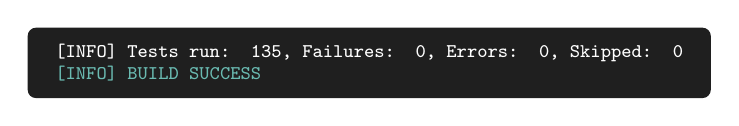
\begin{tikzpicture}
    \node[fill=black!88, text=white, rounded corners=3pt, inner xsep=10pt, inner ysep=6pt, font=\ttfamily\scriptsize, align=left]
      {[INFO] Tests run: 135, Failures: 0, Errors: 0, Skipped: 0\\{\color{ok!70!white}[INFO] BUILD SUCCESS}};
  \end{tikzpicture}
  \vskip8pt
  {\scriptsize\color{muted}Chấm 60 bài: 2,2 giây}
\end{frame}

% ================================================================ 9. Demo
\begin{frame}{Demo}
  \vskip10pt
  {\color{muted}\small Sẽ chứng minh trên màn hình}\par\vskip12pt
  \renewcommand{\arraystretch}{1.75}
  \begin{tabular}{@{}l@{\hspace{10pt}}l@{}}
    \num{1} & Phân quyền nằm ở \textbf{service}, không phải ẩn nút\\
    \num{2} & Luật nghiệp vụ nằm \textbf{trong lớp}, không trong giao diện\\
    \num{3} & Rời cửa sổ bị \textbf{ghi vi phạm}, giờ theo máy chủ\\
    \num{4} & Nộp bài là \textbf{có điểm}, máy thí sinh không chấm\\
    \num{5} & Máy thí sinh \textbf{không đọc được đáp án}, kể cả bằng SQL
  \end{tabular}
\end{frame}

% ================================================================ 10. Tổng kết
\begin{frame}{Tổng kết}
  \begin{columns}[T]
    \begin{column}{0.56\textwidth}
      \vskip6pt
      \renewcommand{\arraystretch}{1.6}
      \begin{tabular}{@{}l@{\hspace{8pt}}l@{}}
        \cmark & \small Phân quyền ở service\\
        \cmark & \small Luật nằm trong lớp\\
        \cmark & \small Vi phạm ghi theo giờ máy chủ\\
        \cmark & \small Có điểm ngay khi nộp\\
        \cmark & \small Máy thí sinh không đọc được đáp án
      \end{tabular}
      \vskip10pt
      {\scriptsize\color{muted}\textbf{Giới hạn:} mọi máy thí sinh dùng chung một tài khoản CSDL;\\
      tách riêng cần máy chủ ứng dụng ở giữa, ngoài công nghệ môn học.}
    \end{column}
    \begin{column}{0.40\textwidth}
      \vskip34pt
      \centering
      {\color{navy}\fontsize{26}{30}\selectfont\bfseries Cảm ơn}\par\vskip6pt
      {\large\color{muted}thầy và các bạn}\par\vskip14pt
      {\color{accent}\rule{1.6cm}{2pt}}\par\vskip10pt
      {\Large\bfseries\color{accent}Hỏi đáp}
    \end{column}
  \end{columns}
\end{frame}

% ================================================================ Dự phòng: ảnh giao diện khi demo hỏng
\newcommand{\shot}[2]{%
  \begin{minipage}[t]{0.485\textwidth}\centering
    \includegraphics[width=\linewidth]{#1}\par\vskip3pt{\scriptsize\color{muted}#2}
  \end{minipage}}
\begin{frame}{Dự phòng · Giảng viên}
  \centering\shot{02-ngan-hang-cau-hoi}{Ngân hàng câu hỏi}\hfill\shot{03-tao-de-theo-ma-tran}{Tạo đề theo ma trận}
\end{frame}
\begin{frame}{Dự phòng · Thí sinh}
  \centering\shot{04-lam-bai}{Làm bài toàn màn hình}\hfill\shot{05-canh-bao-vi-pham}{Cảnh báo rời cửa sổ}
\end{frame}
\begin{frame}{Dự phòng · Đăng nhập và kết quả}
  \centering\shot{01-dang-nhap}{Đăng nhập}\hfill\shot{06-ket-qua-ca-thi}{Kết quả ca thi}
\end{frame}

\end{document}
